\documentclass[aspectratio=169,12pt]{beamer}

\usetheme{Madrid}
\usecolortheme{default}
\setbeamertemplate{navigation symbols}{}
\setbeamertemplate{footline}[frame number]
\setbeamertemplate{caption}[numbered]

\usepackage[T1]{fontenc}
\usepackage[italian]{babel}
\usepackage{amsmath, amssymb}
\usepackage{graphicx}
\usepackage{xcolor}
\definecolor{gscol}{HTML}{0072B2}
\definecolor{lshcol}{HTML}{D55E00}
\graphicspath{{./images/}}

\newcommand{\paper}[1]{{\footnotesize\textcolor{gray}{[#1]}}}

\title[Spike di dark matter e segnali ai telescopi]{Dark matter spikes vicino ai buchi neri galattici\\e il loro impatto sui segnali di DM ai telescopi}
\author{Giovanni Dalena}
\institute[UniBo]{Alma Mater Studiorum -- Universit\`a di Bologna\\Dipartimento di Fisica e Astronomia ``Augusto Righi''\\Corso di Laurea in Fisica\\[4pt]\small Relatore: Prof.\ Filippo Sala}
\date{Anno Accademico 2025/2026}

\begin{document}

\begin{frame}
    \titlepage
\end{frame}

\begin{frame}{Obiettivo della tesi}
    \begin{block}{Domanda}
        Quanto le \textbf{incertezze sul profilo di densit\`a} della dark matter (DM) nella Via Lattea
        influenzano i vincoli di \textbf{rivelazione indiretta} ottenuti dal Centro Galattico?
    \end{block}
    \vspace{6pt}
    \begin{itemize}
        \item Flusso di raggi $\gamma$ $\longrightarrow$ dipende dal profilo tramite il $J$ factor $\propto\!\int\!\rho_{DM}^2\,ds$
        \item Profili diversi $\longrightarrow$ vincoli molto diversi su $\langle\sigma v\rangle$
        \item Crescita adiabatica di Sgr~A* $\longrightarrow$ \textbf{spike} di DM, segnale amplificato
    \end{itemize}
    \vspace{2pt}
    \centering
    {\Large $\Downarrow$}\\[4pt]
    {\small Confrontiamo profili di DM e benchmark di spike con un modello di reliquia termica}
\end{frame}

\begin{frame}{Evidenze astrofisiche}
    \begin{columns}[T]
        \begin{column}{0.56\textwidth}
            \small
            \textbf{Evidenze (tutte gravitazionali)}
            \begin{itemize}
                \item Curve di rotazione piatte
                \item Ammassi di galassie, Bullet Cluster
                \item CMB e strutture a grande scala: $\Omega_{DM}\simeq 0.264$
            \end{itemize}
            \vspace{6pt}
            \textbf{Candidato: WIMP}
            \begin{itemize}
                \item Massa GeV--TeV
                \item \emph{Freeze-out} termico $\Rightarrow$ \emph{WIMP miracle}
                \[
                \langle\sigma v\rangle \simeq 3\times10^{-26}\ \mathrm{cm^3/s}
                \]
            \end{itemize}
        \end{column}
        \begin{column}{0.44\textwidth}
            \centering
            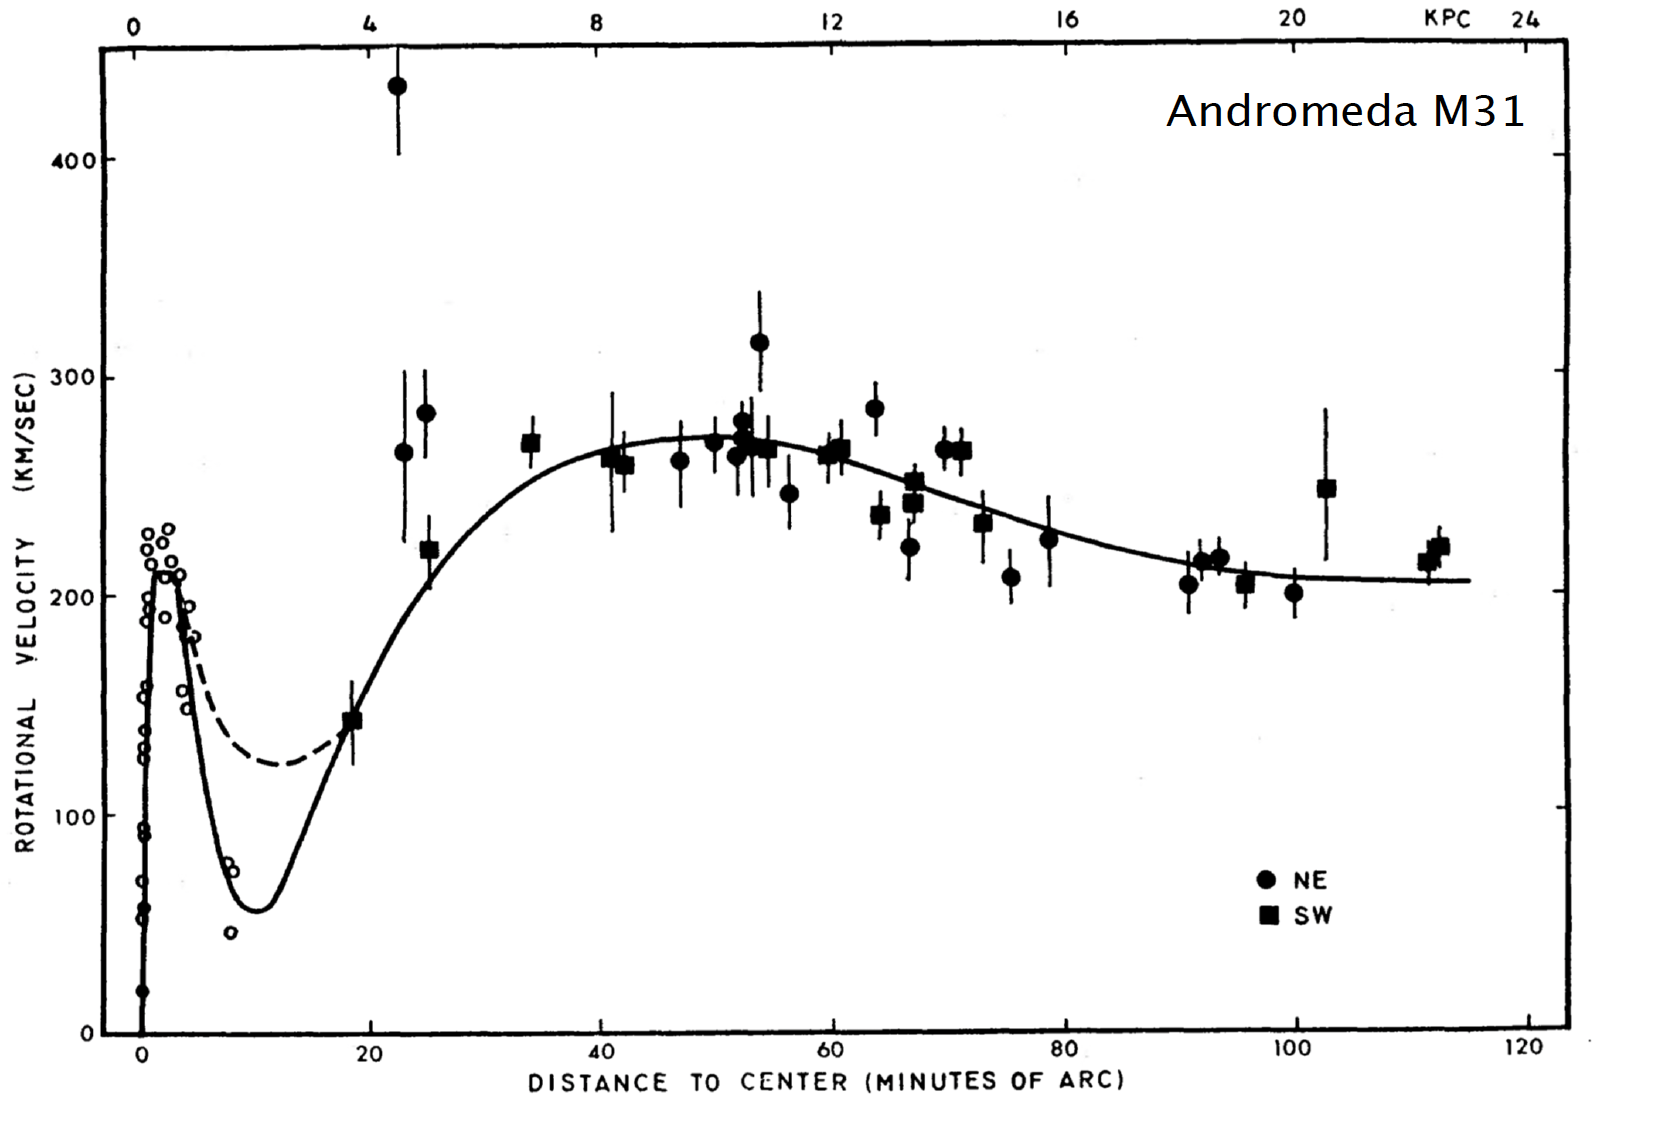
\includegraphics[width=\textwidth]{RCM31.png}\\[3pt]
            {\tiny Curva di rotazione di M31 (Rubin \& Ford, 1970)}
        \end{column}
    \end{columns}
\end{frame}

\begin{frame}{Rivelazione indiretta}
    \small
    Il flusso di raggi $\gamma$ da annichilazione di DM si fattorizza come:
    \[
    \frac{d\Phi_\gamma}{d\Omega\,dE}
    =
    \underbrace{\frac{\langle\sigma v\rangle}{8\pi M_{DM}^2}\frac{dN_\gamma}{dE}}_{\text{fisica delle particelle}}
    \times
    \underbrace{\int_{\text{l.o.s.}} \!\! ds\ \rho_{DM}^2}_{\displaystyle J \text{ factor}}
    \]
    \begin{itemize}
        \item $J$ factor $\longrightarrow$ contiene \textbf{tutta} l'informazione astrofisica
        \item Integrale di $\rho_{DM}^{\,2}$ lungo la linea di vista
        \item[$\Rightarrow$] tutta l'incertezza astrofisica sui vincoli passa da $J$
    \end{itemize}
    \vspace{-6pt}
    \begin{block}{Target}
        {\small\textbf{Centro Galattico}: segnale atteso molto intenso ma fondo astrofisico elevato e non del tutto compreso}
    \end{block}
\end{frame}

\begin{frame}{Profili di DM al Centro Galattico}
    \small
    Profili rappresentativi:
    \[
    \text{Einasto (piccato)} \quad\longleftrightarrow\quad \text{NFW} \quad\longleftrightarrow\quad \text{Burkert (cored)}
    \]
    Parametri fissati da $\rho(r_\odot)=0.4~\mathrm{GeV/cm^3}$ e $M(<60~\mathrm{kpc})=4.7\times10^{11}M_\odot$.
    \vspace{2pt}
    \begin{center}
    $J$ integrato su
    $\Omega_{\mathrm{obs}}=\Omega(\theta<1^\circ,\ |b|>0.3^\circ)$
    \end{center}
    \vspace{-2pt}
    \begin{table}
    \centering
    \small
    \resizebox{\textwidth}{!}{%
    \begin{tabular}{c|c|c|c|c|c}
    \hline
     & Einasto & Burkert & $\mathrm{NFW}_{30\,\mathrm{pc}}$ & $\mathrm{NFW}_{300\,\mathrm{pc}}$ & $\mathrm{NFW}_{3\,\mathrm{kpc}}$ \\
    \hline
    $\log_{10}\!\big(J_{\Omega_{\mathrm{obs}}}\,[\mathrm{GeV^2/cm^5}]\big)$
    & 21.96 & 19.35 & 21.57 & 21.16 & 19.77 \\
    \hline
    \end{tabular}}
    \end{table}
    \vspace{4pt}
    \begin{itemize}
        \item Einasto presenta un $J$ factor più di 2 ordini di grandezza maggiore rispetto a Burkert, 
        fornirà quindi limiti più stringenti su $\langle\sigma v\rangle$
    \end{itemize}
\end{frame}

\begin{frame}{Limiti sulla sezione d'urto}
    \small
    \textbf{Modello}: $\chi\chi\to\phi\phi\to W^+W^-\,W^+W^-$
    \begin{columns}[T]
        \begin{column}{0.34\textwidth}
            \small
            \begin{itemize}
                \item Reliquia termica:
                $\langle\sigma v\rangle = 2.2\times10^{-26}~\mathrm{cm^3/s}$
                \item Limiti H.E.S.S.\ al 95\% C.L.\ sulla regione
                $0.5^\circ<\theta<3^\circ$, $|b|>0.3^\circ$
            \end{itemize}
            \vspace{2pt}
            \begin{block}{Risultato}
                \textbf{Nessuna massa esclusa}, nè per NFW nè per il cored
            \end{block}
        \end{column}
        \begin{column}{0.66\textwidth}
            \centering
            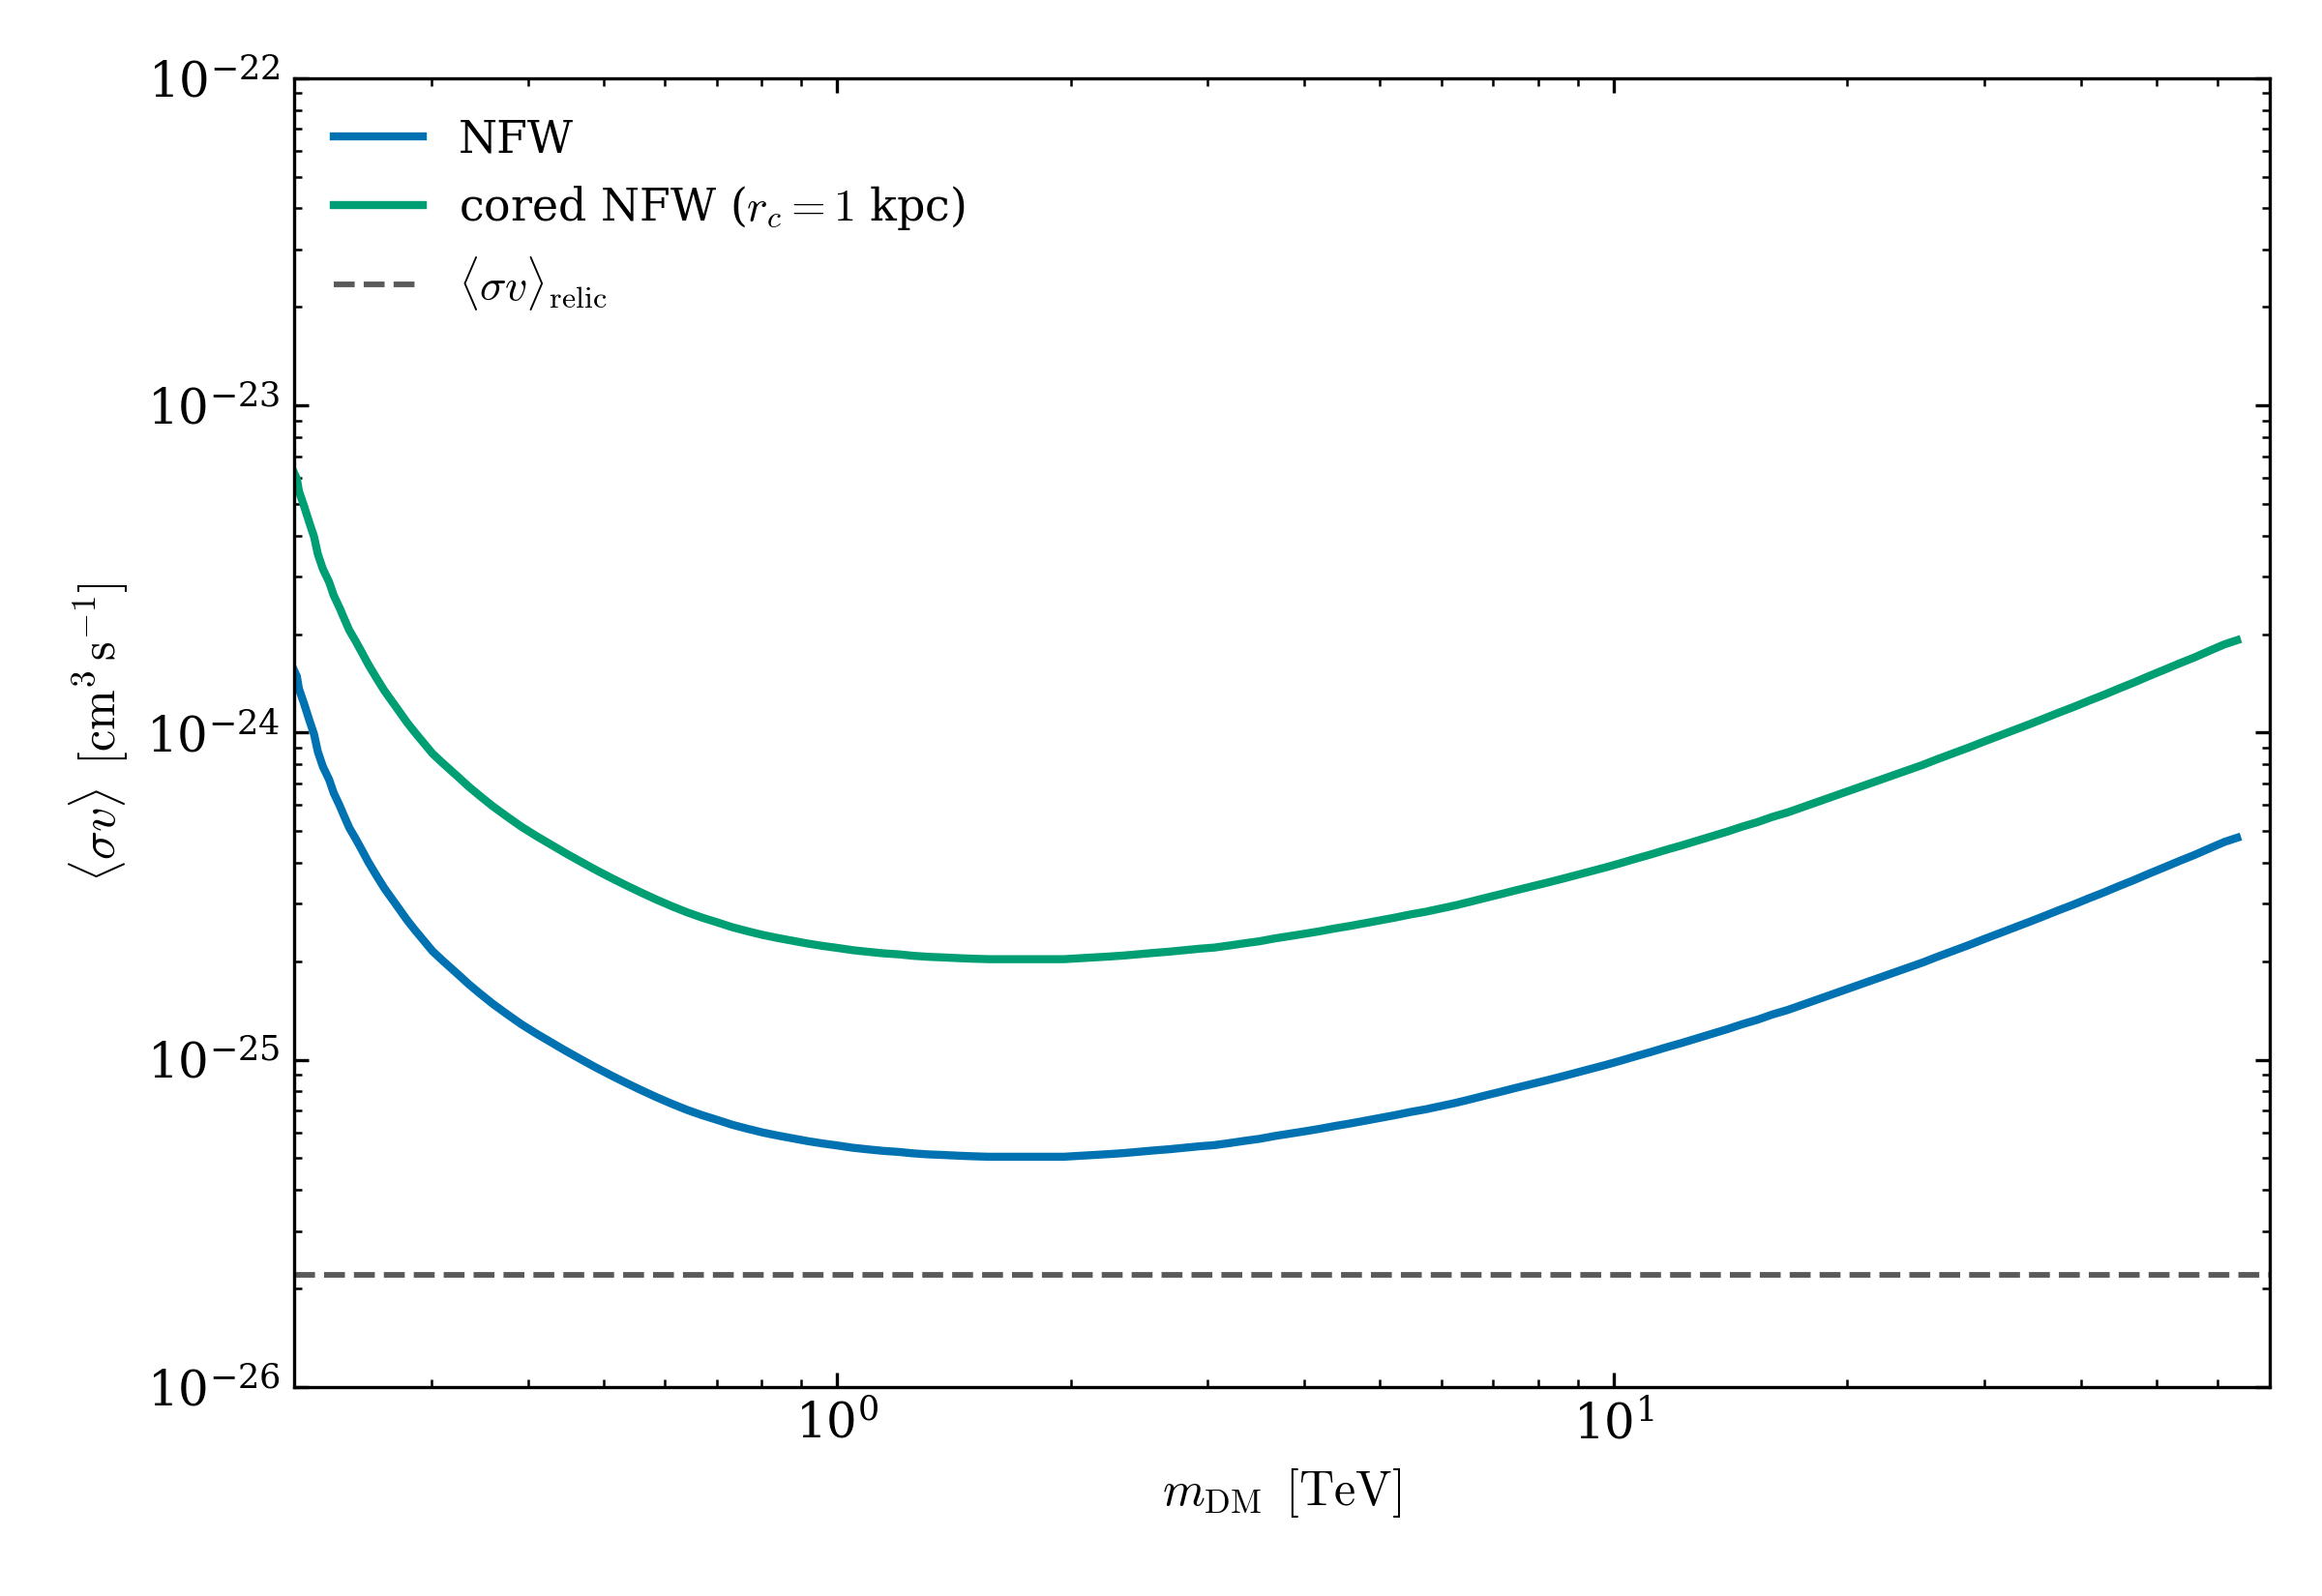
\includegraphics[width=\textwidth,height=0.70\textheight,keepaspectratio]{Sigmav_limits.png}
        \end{column}
    \end{columns}
    \vspace{2pt}
    {\footnotesize Punto escluso $\Rightarrow$ profilo, $m_{DM}$, $\langle\sigma v\rangle$ \emph{simultaneamente} incompatibili.}
\end{frame}

\begin{frame}{Crescita adiabatica e formazione della spike}
    \small
    \textbf{Sgr~A*}: $M_{BH}=(4.15\pm0.01)\times10^6\,M_\odot$ \paper{GRAVITY 2019}
    \vspace{6pt}
    \begin{itemize}
        \item Crescita del BH \emph{lenta} rispetto al tempo orbitale della DM $\Longrightarrow$ regime \textbf{adiabatico}
        \item Si conservano momento angolare $L$ e azione radiale $I_r$
        \item Teorema di Liouville: $f'(E',L')=f(E,L)$
    \end{itemize}
    \vspace{6pt}
    \begin{block}{Conseguenza}
        La DM \textbf{non viene creata}: viene solo \textbf{redistribuita} verso il centro
        $\Longrightarrow$ cuspide molto densa, la \textbf{spike}.
    \end{block}
    \vspace{4pt}
    \centering
    {\small Annichilazione $\propto\rho_{DM}^2$ $\Longrightarrow$ amplificazione enorme del segnale}
\end{frame}

\begin{frame}{Pendenza della spike e saturazione}
    \begin{columns}[T]
        \begin{column}{0.42\textwidth}
            \footnotesize
            Halo $\rho\propto r^{-\gamma}$ $\Longrightarrow$ spike $\rho_{sp}\propto r^{-\gamma_{sp}}$:
            \[
            \boxed{\;\gamma_{sp}=\frac{9-2\gamma}{4-\gamma}\;}
            \qquad {\scriptstyle 0<\gamma<2}
            \]
            \begin{itemize}
                \item NFW ($\gamma=1$) $\Rightarrow \gamma_{sp}=7/3$
                \item Cored ($\gamma_c=0.4$) $\Rightarrow \gamma_{sp}\simeq2.28$
                \item Per $\gamma=0$ esatto la formula non vale
            \end{itemize}
            \vspace{4pt}
            \textbf{Saturazione} da annichilazione:
            \[
            \rho_{\rm core}=\frac{m_{DM}}{\langle\sigma v\rangle\,t_{BH}}
            \simeq 1.4\times10^{11}\ \frac{\rm GeV}{\rm cm^3}
            \]
            {\scriptsize $m_{DM}=1$~TeV, $t_{BH}\simeq10^{10}$~yr (conservativo)}
        \end{column}
        \begin{column}{0.58\textwidth}
            \centering
            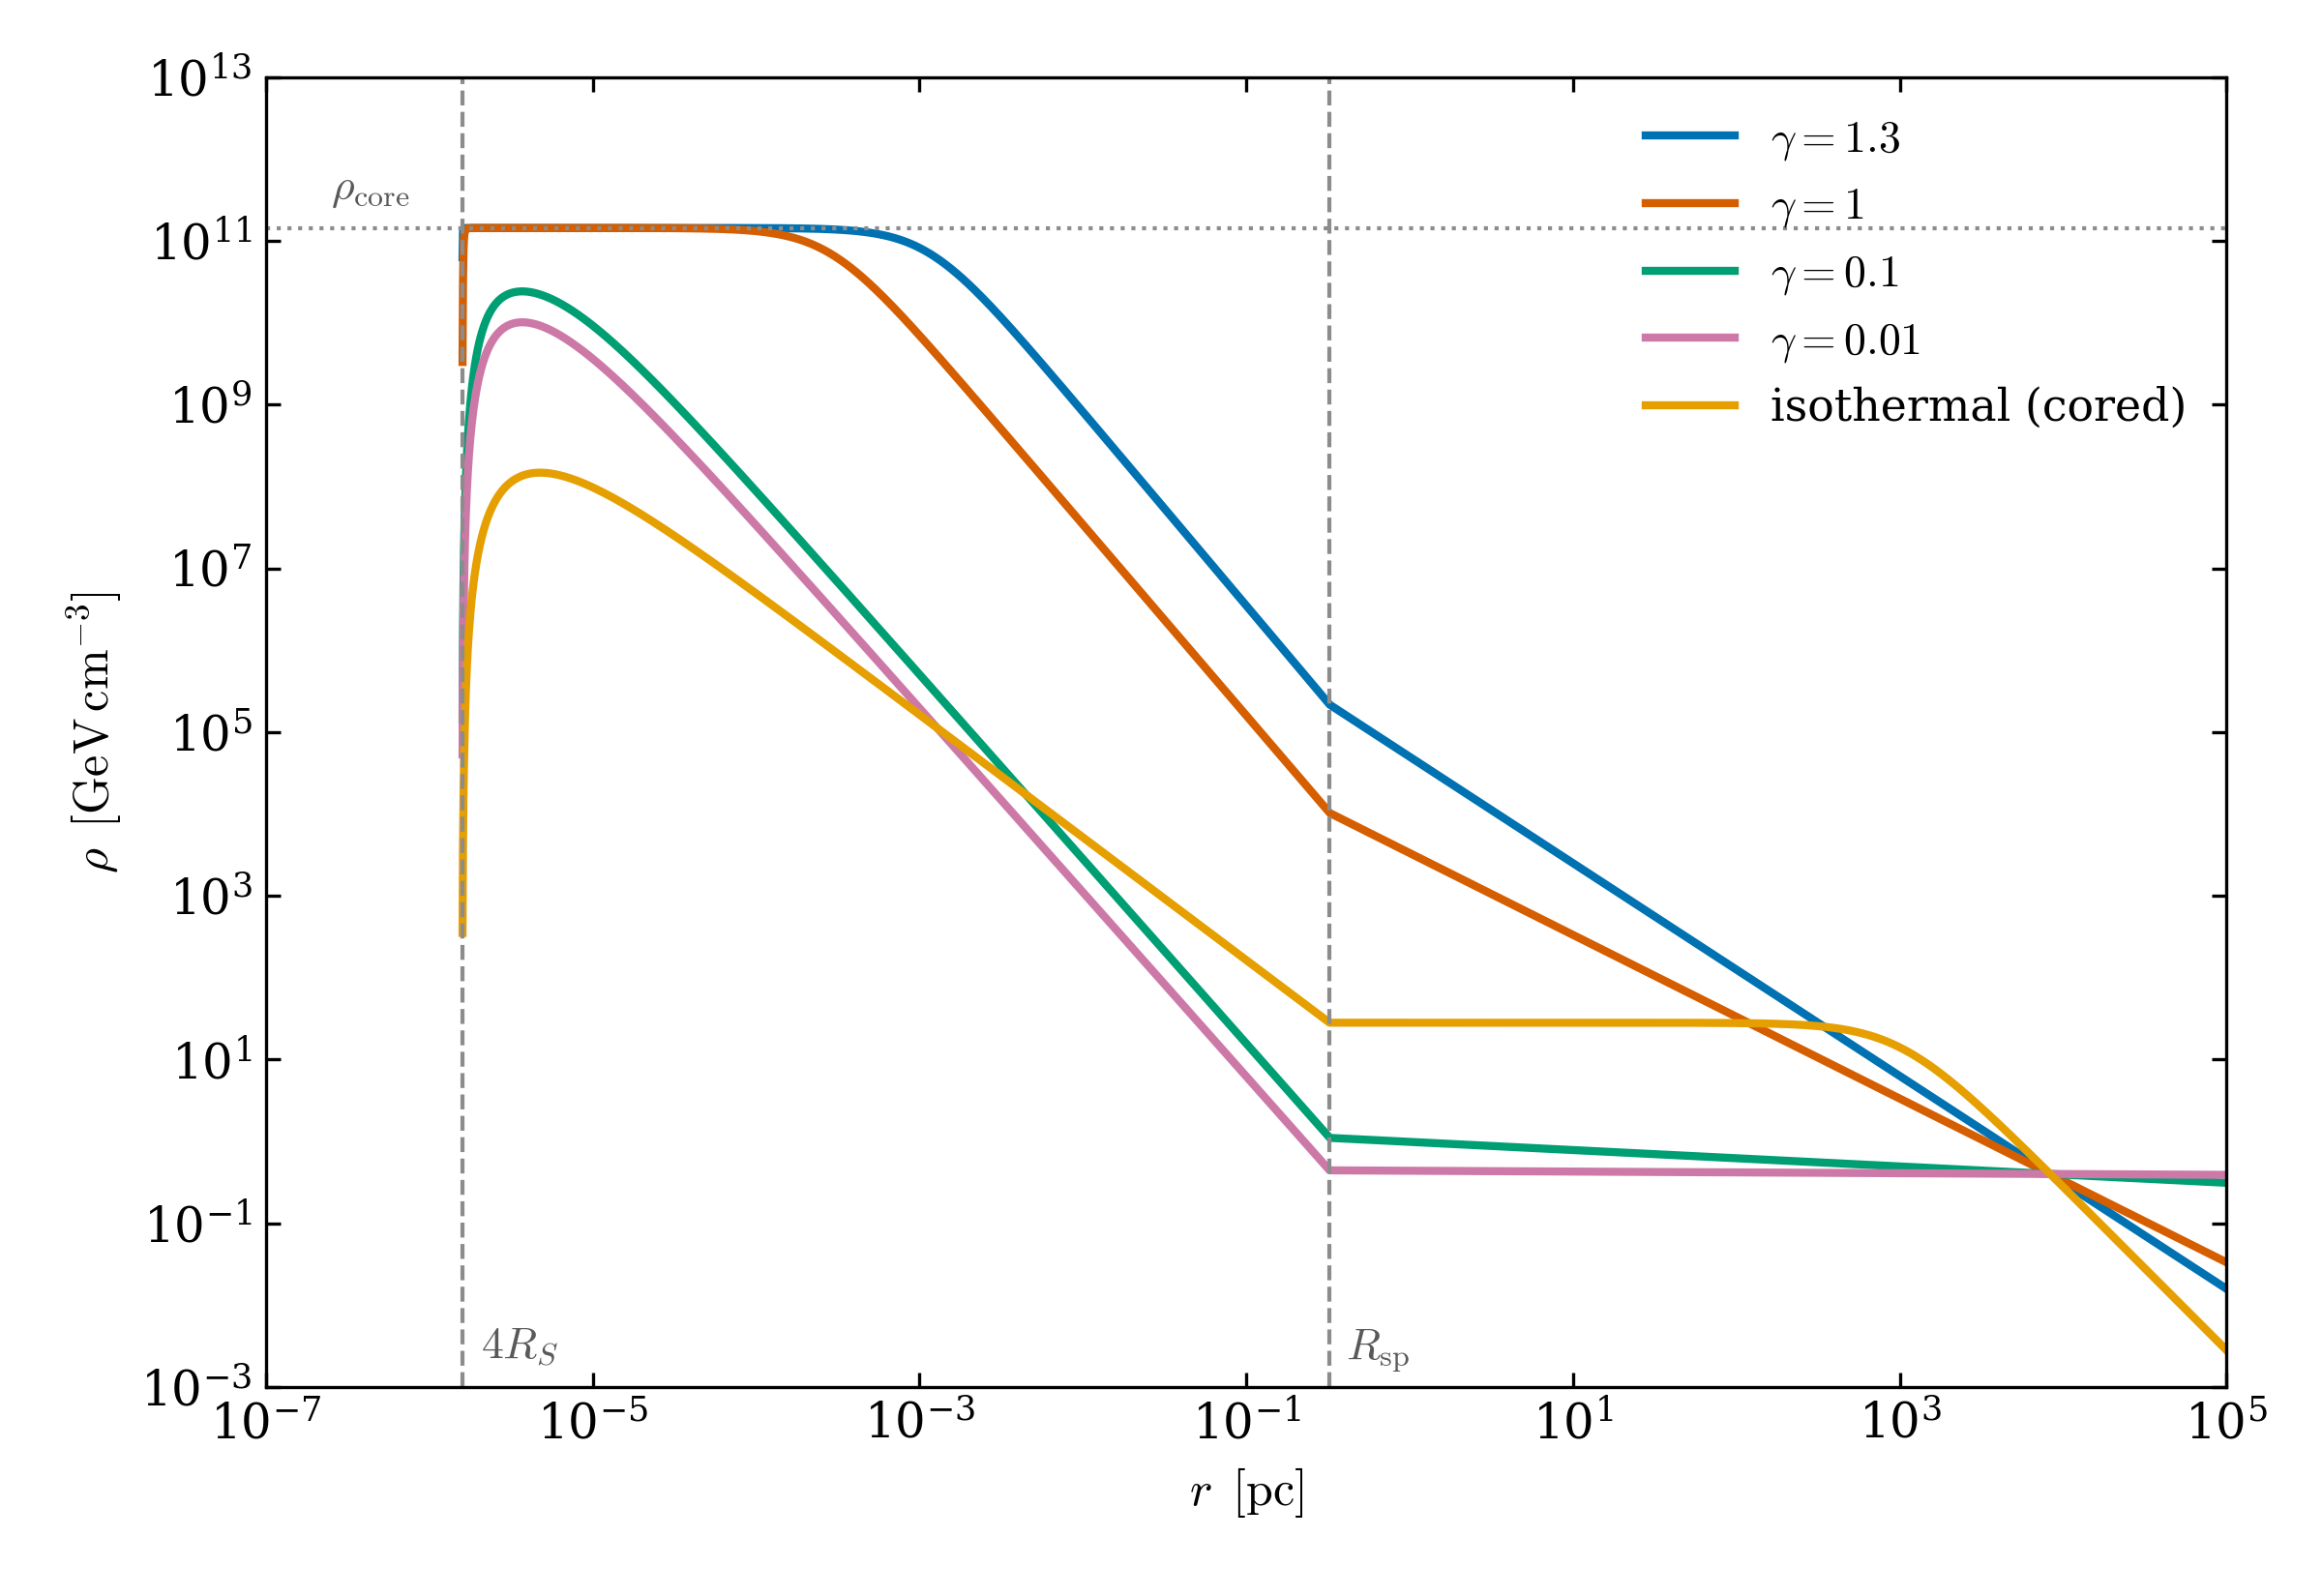
\includegraphics[width=\textwidth,height=0.94\textheight,keepaspectratio]{Spike_slope.png}
        \end{column}
    \end{columns}
\end{frame}

\begin{frame}{Spike benchmark}
    \begin{columns}[T]
        \begin{column}{0.36\textwidth}
            \footnotesize
            Pendenza $\gamma$ di $\rho\propto r^{-\gamma}$:
            \vspace{4pt}
            \begin{center}
            \begin{tabular}{l|c|c}
            \hline
             & \textbf{NFW} & \textbf{cored} \\
            \hline
            Alone ($r>R_{\rm sp}$) & $1$ & $0.4$ \\
            \hline
            \textbf{GS} ($r<R_{\rm sp}$) & $7/3$ & $2.28$ \\
            \hline
            \textbf{LSH} ($r>r_b$) & $3/2$ & $3/2$ \\
            \textbf{LSH} ($r<r_b$) & $7/3$ & $2.28$ \\
            \hline
            \end{tabular}
            \end{center}
            \vspace{4pt}
            $R_{\rm sp}\simeq0.32$~pc \qquad $r_b=0.01$~pc
        \end{column}
        \begin{column}{0.64\textwidth}
            \centering
            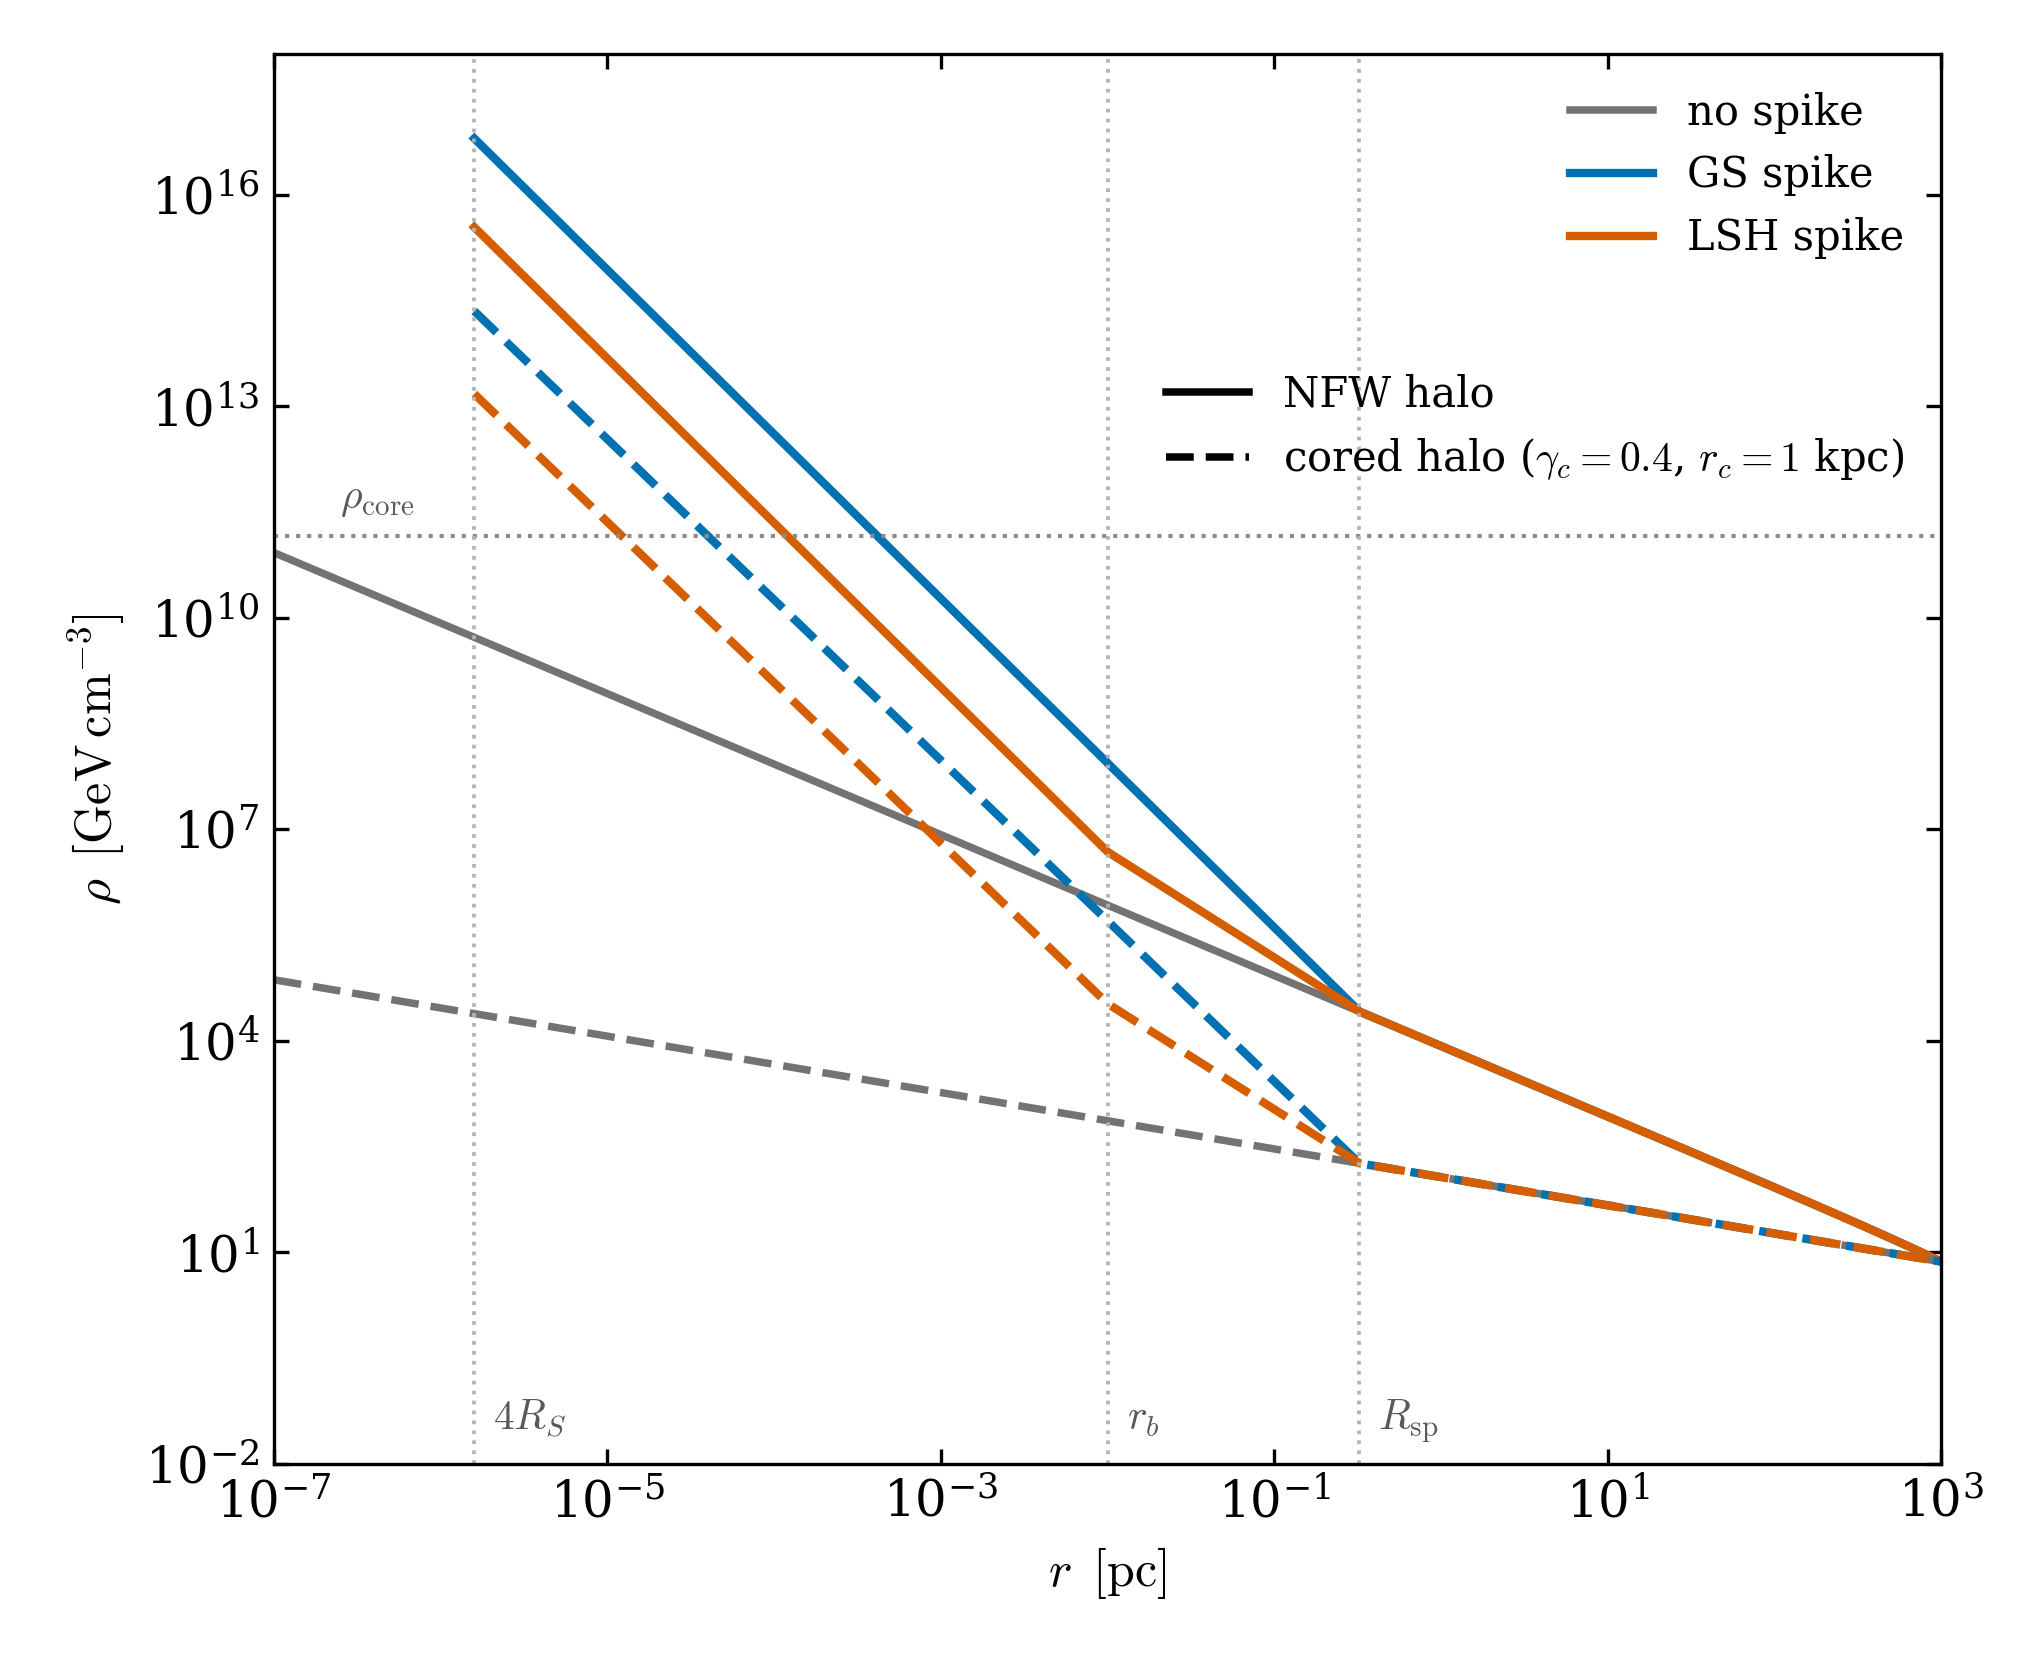
\includegraphics[width=\textwidth,height=0.82\textheight,keepaspectratio]{Spike_profiles.png}
        \end{column}
    \end{columns}
\end{frame}

\begin{frame}{$J$ factors con spike}
    \small
    $J$ factor sul pixel centrale $0.1^\circ\times0.1^\circ$ su Sgr~A*:
    \begin{table}
    \centering
    \resizebox{\textwidth}{!}{%
    \begin{tabular}{c|c|c|c||c|c|c}
    \hline
    $\log_{10}\!\big(J_{0.1^\circ\times0.1^\circ}\,[\mathrm{GeV^2/cm^5}]\big)$
    & NFW & NFW$+$GS & NFW$+$LSH & Core & Core$+$GS & Core$+$LSH \\
    \hline
    $\langle\sigma v\rangle \to 0$
    & 20.70 & \textbf{27.74} & 25.22 & 18.63 & 22.87 & 20.53 \\
    \hline
    $\langle\sigma v\rangle = 2.2\times10^{-26}~\mathrm{cm^3/s}$
    & 20.70 & 23.62 & 22.02 & 18.63 & 20.60 & 19.19 \\
    \hline
    \end{tabular}}
    \end{table}
    \vspace{8pt}
    \begin{block}{Gerarchia delle incertezze}
        Profilo interno dell'halo ($\sim\!5$ ordini) $\gg$ forma della spike ($\sim\!2$ ordini).
    \end{block}
\end{frame}

\begin{frame}{Impatto della spike sui limiti}
    \begin{columns}[T]
        \begin{column}{0.24\textwidth}
            \small
            \textbf{Masse escluse}
            \vspace{10pt}

            {\color{gscol}\rule[0.15em]{1.4em}{3pt}}\ \textbf{GS}\\[3pt]
            \hspace*{0.2em}$0.3$--$100$~TeV\\[1pt]
            \hspace*{0.2em}{\scriptsize (tutto il range)}
            \vspace{12pt}

            {\color{lshcol}\rule[0.15em]{1.4em}{3pt}}\ \textbf{LSH}\\[3pt]
            \hspace*{0.2em}$15$--$69$~TeV
        \end{column}
        \begin{column}{0.76\textwidth}
            \centering
            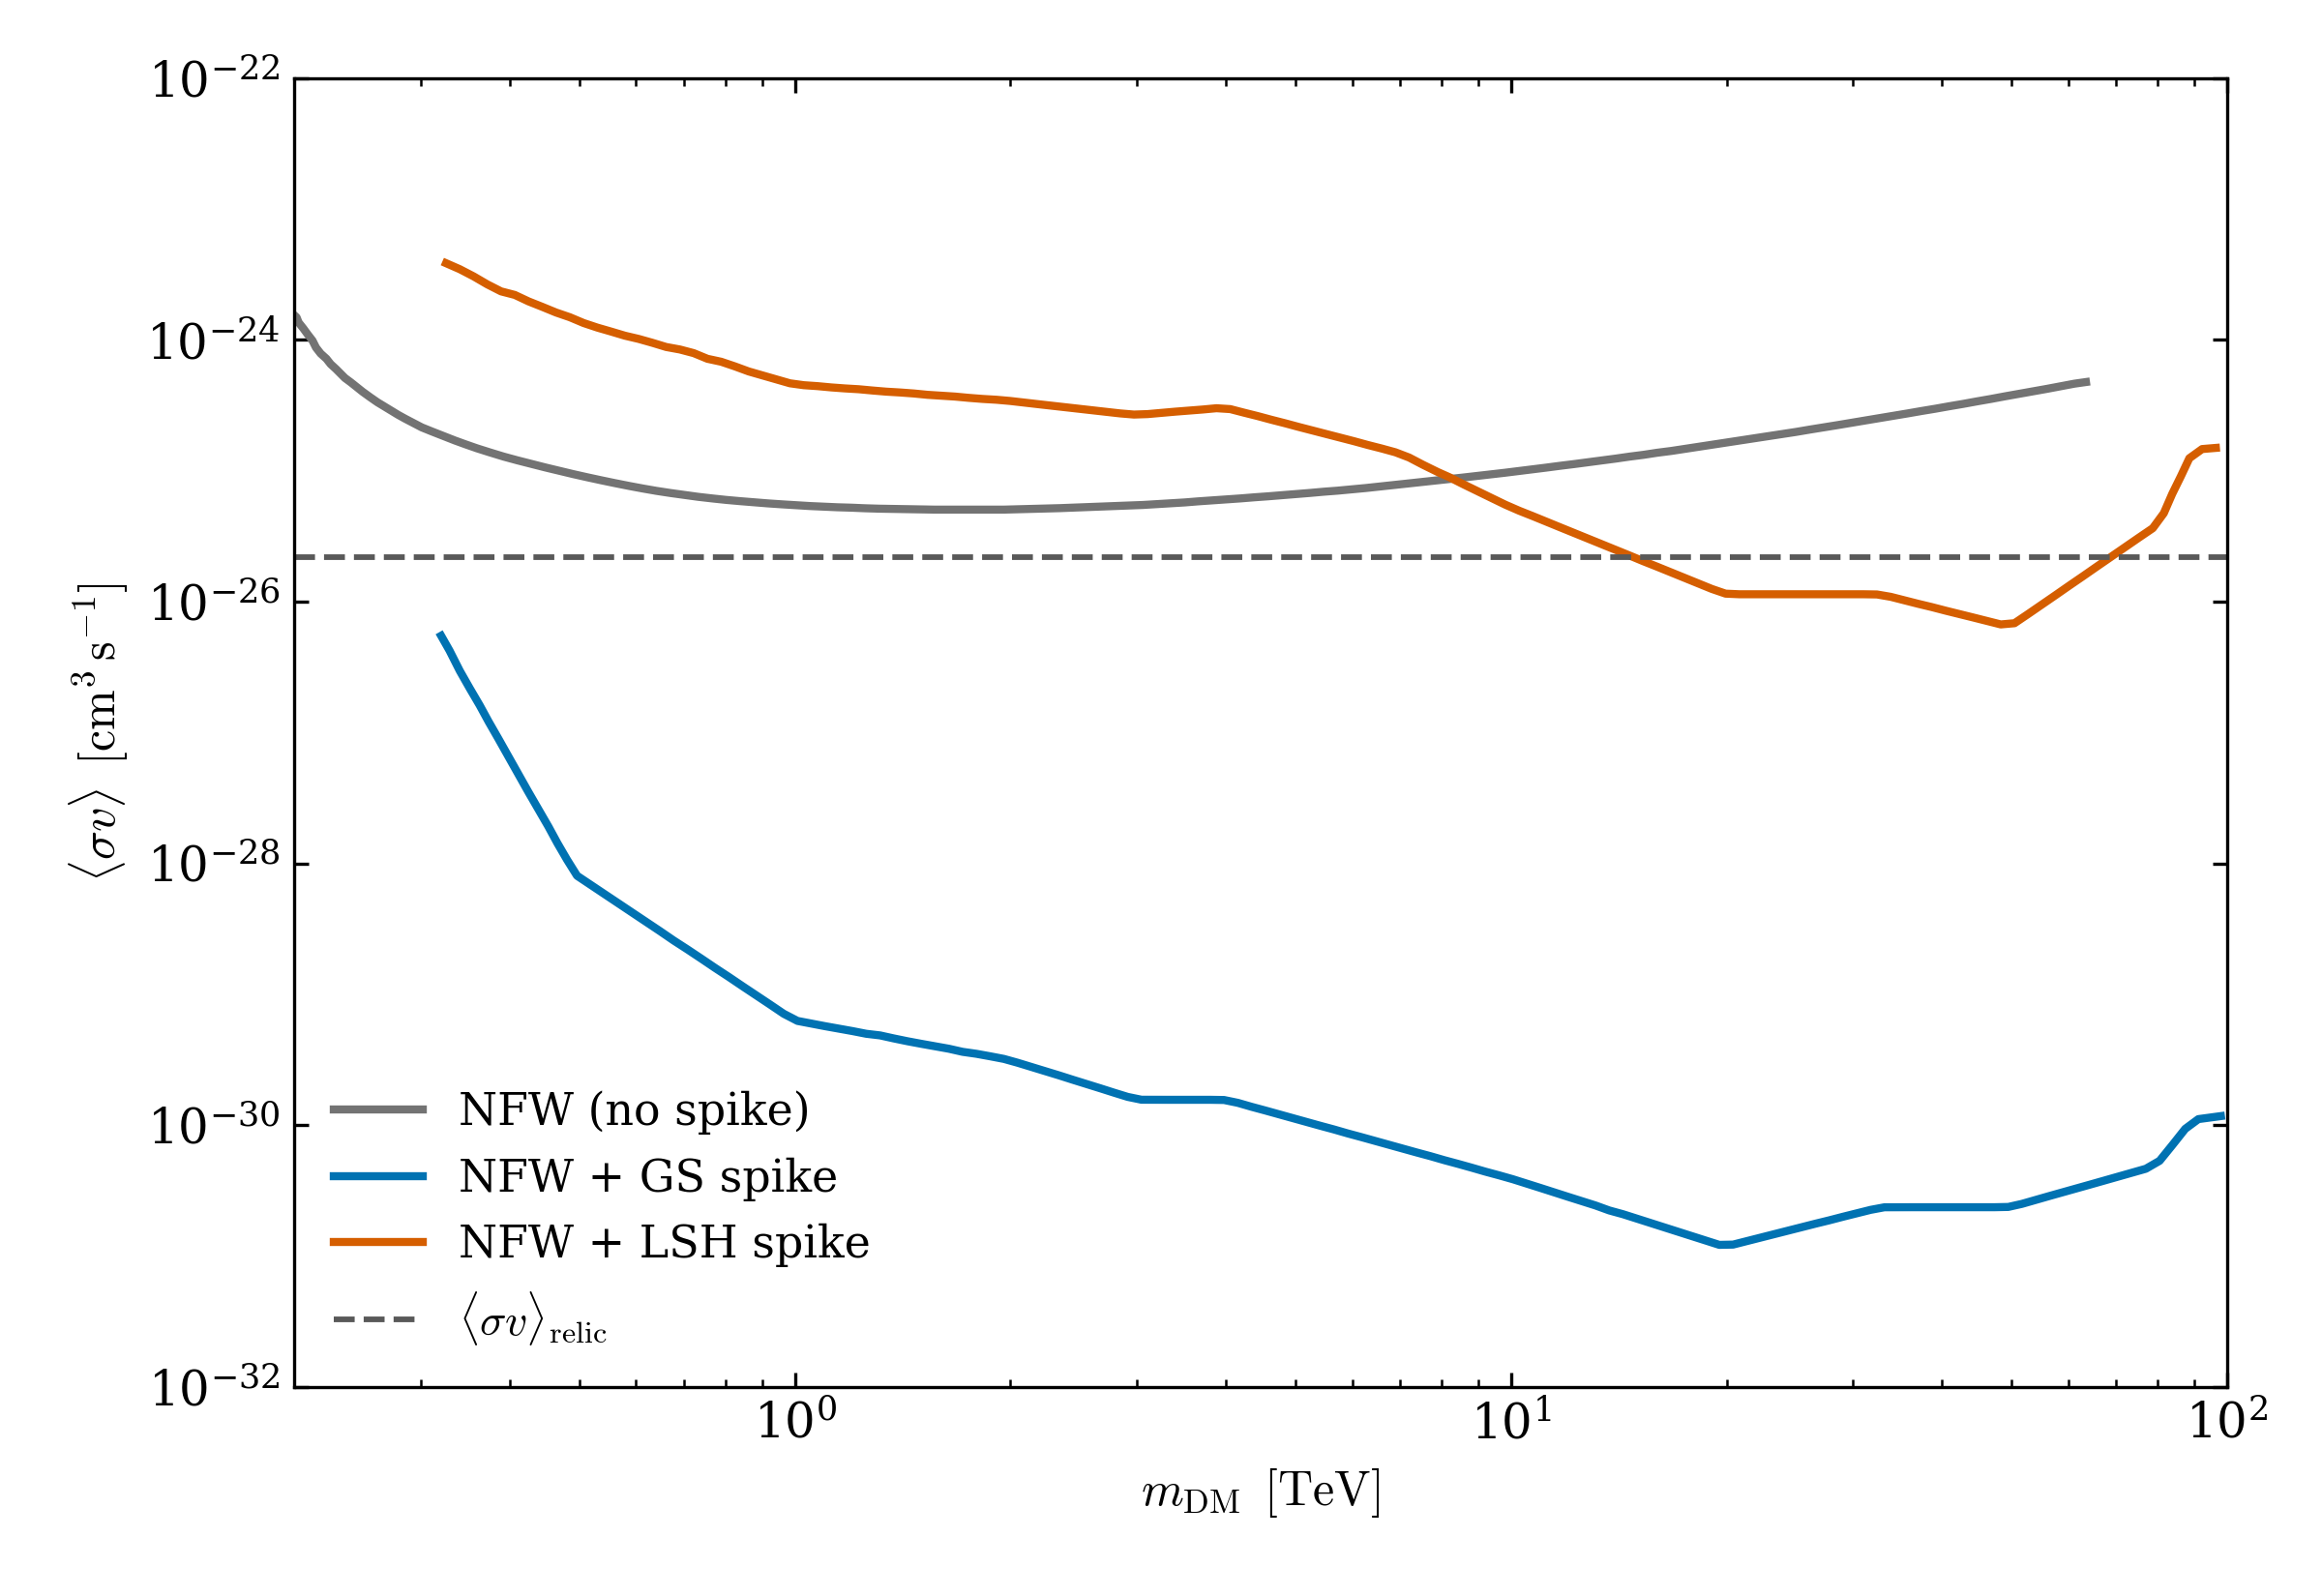
\includegraphics[width=\textwidth,height=0.82\textheight,keepaspectratio]{Sigmav_limits_spike.png}
        \end{column}
    \end{columns}
\end{frame}

\begin{frame}{Conclusioni}
    \begin{itemize}
        \item Vincoli su $\langle\sigma v\rangle$ $\longrightarrow$ dipendono \textbf{criticamente} da profilo interno e benchmark di spike
        \item A parità di halo NFW, la sola scelta della spike sposta la regione esclusa
        da tutto il range (GS) a una finestra $15$--$69$~TeV (LSH)
        \item Nei punti esclusi $\Longrightarrow$ halo interno più piatto,
        oppure spike attenuata, oppure mai formata
    \end{itemize}
    \vspace{6pt}
    \begin{block}{Messaggio}
        Le osservazioni del Centro Galattico sondano non solo le propriet\`a della DM,
        ma anche la \textbf{storia dinamica} della regione pi\`u interna della Via Lattea.
    \end{block}
    \vfill
    \centering
    {\large Grazie per l'attenzione}
\end{frame}

\end{document}
